% 第5章 低速飛行特性
%!TEX root = main.tex

%%%%%%%%%%%%%%%%%%%%%%
\chapter{低速飛行特性}
\label{flight_char}
%%%%%%%%%%%%%%%%%%%%%%

本章では,実験で得られたデータから,これまでに述べた力学モデルを用いてパラメータ同定を行ない,低速飛行時の飛行特性について検証する.まず機体が持つ固有振動をとらえるために,線形モデルによる固有値解析を行なう.次に,同定を行なった結果から,設定した空気力モデルの妥当性を検討する.最後に,同定結果をCFD解析の結果と比較し,考察を行なう.

%%%%%%%%%%%%%%%%%%%%%%%%%%%%%%%%%%%%
\section{線形モデルによる固有値解析}
\label{sec:analyze}
%%%%%%%%%%%%%%%%%%%%%%%%%%%%%%%%%%%%

本節では,線形化された機体の飛行モデルを用いて,固有値解析を行なう.まず,式(\ref{eq:lin_model})より,$\Delta$を省略して微分方程式をまとめると
\begin{equation}
  \dfrac{d}{dt}
  \underbrace{
  \left[
  \begin{array}{cccc}
    u \\
    \alpha \\
    q \\
    \theta \\
  \end{array}
  \right]}_{\underline{x}} =
  \underbrace{
  \left[
  \begin{array}{cccc}
    X_u & X_\alpha & X_q & X_\theta \\
    \overline{Z_u} & \overline{Z_\alpha} & \overline{Z_q} & \overline{Z_\theta} \\
    \overline{M_u} & \overline{M_\alpha} & \overline{M_q} & \overline{M_\theta} \\
    0 & 0 & 1 & 0
  \end{array}
  \right]}_{A}
  \underbrace{
  \left[
  \begin{array}{cccc}
    u \\
    \alpha \\
    q \\
    \theta \\
  \end{array}
  \right]}_{\underline{x}} +
  \underbrace{
  \left[
  \begin{array}{cccc}
    X_{\delta_e} & X_{T_m} & 0 & 0 \\
    \overline{Z_{\delta_e}} & \overline{Z_{T_m}} & \overline{Z_{T_r}} & \overline{Z_{T_f}} \\
    \overline{M_{\delta_e}} & \overline{M_{T_m}} & \overline{M_{T_r}} & \overline{M_{T_f}} \\
    0 & 0 & 0 & 0
  \end{array}
  \right]
  \left[
  \begin{array}{cccc}
    \delta_e \\
    T_m \\
    T_r \\
    T_f \\
  \end{array}
  \right]}_{\underline{u}}
\end{equation}
となる.プロセスノイズを省略すれば,\cite{}を参考に,この状態方程式は行列$A$と状態量$\underline{x}(u,\alpha,q,\theta)$,入力$\underline{u}(\delta_e,T_m,T_r,T_f)$を用いることによって
\begin{equation}
  \dfrac{d\underline{x}}{dt} = A\underline{x} + \underline{u}
\label{eq:matrix_A}
\end{equation}
と表すことができる.ここで入力$\underline{u}$が,振動や減衰を表す関数
\begin{equation}
  \underline{u} = \sum \underline{f} e^{\omega t}
\end{equation}
であるとする.ただし$\omega$は複素数($\omega \in \mathbb{C}$)である.これにより,状態量$\underline{x}$は解析的に解くことができ
\begin{equation}
  \underline{x} = \left(\sum_{i}C_i x_i e^{\lambda_i t}\right) +
  \sum(\omega I - A)^{-1} \underline{f} e^{\omega t}
\end{equation}
となる.ここで右辺第1項は,ある係数$C_i$,行列$A$の固有値$\lambda_i$,固有ベクトル$x_i$で表された一般解で,状態に固有な振動や発散,減衰などを表している.右辺第2項は特殊解であり,入力と同じ周波数成分を持つ.つまり,外乱がない限り,状態量は周波数成分として固有振動数や入力に存在する周波数成分に相関するということである.

そこで,\ref{sec:filter}でも述べたように,固有振動数を計算することで機体の運動が持つおおよその周波数帯をつかみ,データのフィルタリングに利用する.実際に式(\ref{eq:matrix_A})の行列$A$について,固有値を計算して絶対値をプロットしたものがFig. \ref{fig:eigenvalue}である.ただし,実験中の風の影響などの外乱が大きいと思われるデータは除き,計算を行なった.行列$A$が4次の正方行列であるため,各データ点ごとに最大4つの固有値を持ち,それぞれ色分けされている.グラフ内の縦線は,複数の実験データそれぞれの境界を示す.

Fig. \ref{fig:eigenvalue}から,機体の回転翼機モードにおける低速飛行縦運動の固有振動数は,おおよそ0〜5$\mathrm{[Hz]}$であることが見て取れる.つまり,この範囲内の周波数はフィルタリングなどの処理で落としてはいけない.このように小型UAVにおいても,運動の固有値解析を行なうことは有用であると考えられる.

\begin{figure}[H]
	\centering
	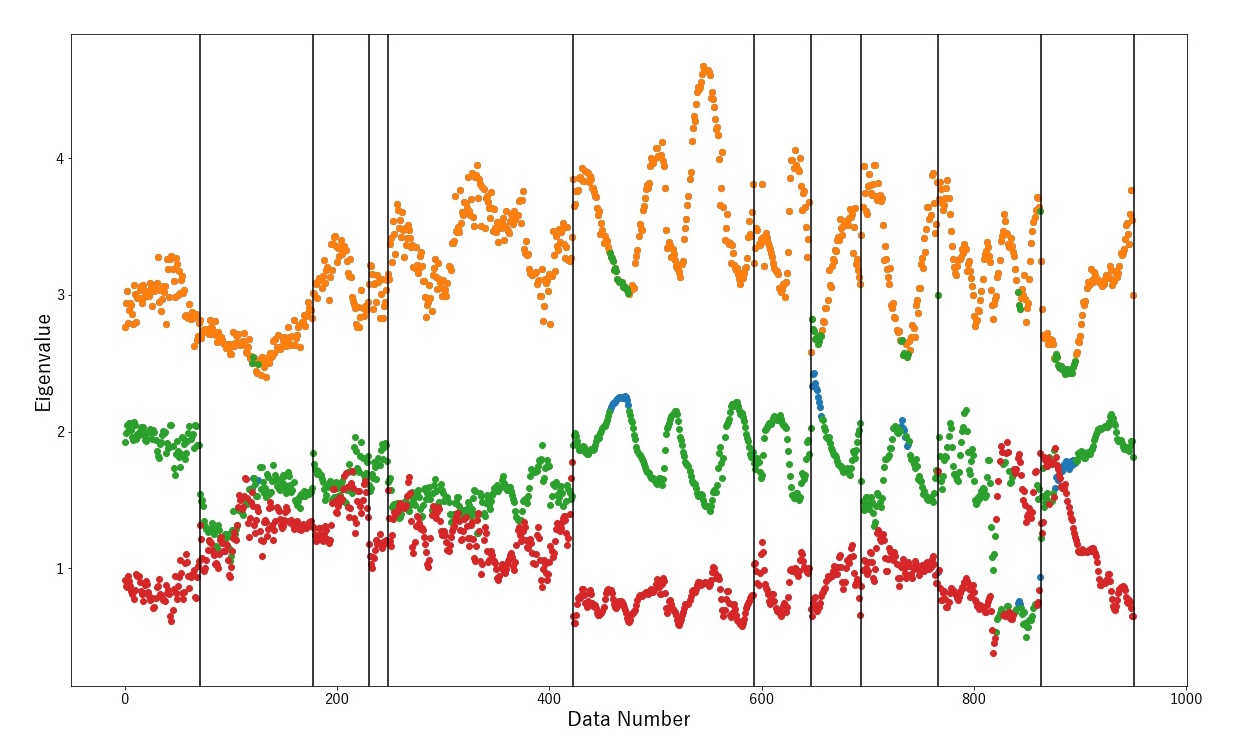
\includegraphics[clip,width=15.0cm,bb=0 0 1250 750]{./z_figure_files/chapter5/1_eigenvalue.jpeg}
	\caption{Eigenvalue of matrix A}
	\label{fig:eigenvalue}
\end{figure}

%%%%%%%%%%%%%%%%%%%%%%%%%%%%
\section{空気力モデルの検証}
%%%%%%%%%%%%%%%%%%%%%%%%%%%%

本節では,パラメータ同定の結果から,式(\ref{eq:L})〜(\ref{eq:Cm})で設定した空気力モデルおよび空力係数が妥当であるかを考える.まず,$L,D,M_a$のモデルについて検証する.Fig. \ref{fig:}に示すように,同定結果から算出したそれぞれの空力係数を,$L_{log},D_{log},M_{a_{log}}$から算出したそれぞれの空力係数と比較する.ただし,式(\ref{eq:CL}),~(\ref{eq:Cm})より空力係数に関係する変数は,$\alpha,\dot{\alpha},q,\delta_e,V_a$の計5個あるため,その中から代表して$V_a$を横軸にとった射影を図示している.

%%%%%%%%%%%%%%%%%%%%%%%%%%%%%%%
\section{CFDによる解析結果との比較}
%%%%%%%%%%%%%%%%%%%%%%%%%%%%%%%
